\textbf{Ejemplo 1:}\\

Una industria solicita 8.000.000 COP al banco para pagarlos en 20 pagos trimestrales comenzando con estos 1 año después de concedido el préstamo. Calcular el valor de la cuota trimestral a cancelar, tenga en cuenta que la tasa de interés es del 36\% nominal anual trimestre vencido.\\

%%%%%%%%%%%%%%%%%%% EJERCICIO 1 %%%%%%

%\newpage %USAR SOLO SI EL SOLUCIÓN QUEDA SOLO Y ES NECESARIO BAJARLO A LA SIGUIENTE PAGINA
\textbf{Solución.}
% Se debe definir el cero de la serie uniforme, como se maneja de manera vencida el cero estará en el periodo 3 en el diagrama de flujo logrando así que el primer pago se realicé en el periodo 4 que es cuando se completa un año, según el enunciado se desea realizar el primer pago un año después de realizado el préstamo.\\
% \\
% Para que se tengan los 20 pagos deseados entonces al comenzar en el periodo 3 se debe terminar en el periodo 23, así se tendrán los 20 pagos desde el periodo 4 hasta el periodo 23 (tener en cuenta que son periodos trimestrales vencidos).\\
% \\
% Como deseamos trasladar el nuevo valor presente al periodo focal entonces tomamos un \textbf{n1} como n1 = 3 ptv para calcular el valor presente nuevo que se tendrá al momento de iniciar los pagos ya que a pesar de que no se realiza el pago este si se ve afectado por el interés.\\
% \\
% Luego tendremos un \textbf{n2}  pero teniendo en cuenta el nuevo cero y con el nuevo VP, con esto tendremos un n2 = 20 ptv\\
%La tabla irá centrada
\begin{center}
	\renewcommand{\arraystretch}{1.5}% Margenes de las celdas
	%Creación de la cuadricula de 3 columnas \end{flushleft}
	\begin{longtable}[H]{|c|c|c|}
		%Creamos una linea horizontal
		\hline
		%%%%%%%%%% INICIO TITULO 	
		%Lo que se hace aquí es mezclar las 3 columnas en una sola
		\multicolumn{3}{|c|}{\cellcolor[HTML]{FFB183}\textbf{1. Asignación del periodo focal}}   \\ \hline
		\multicolumn{3}{|c|}{$pf=0 ptv$}\\ \hline
		\multicolumn{3}{|c|}{\cellcolor[HTML]{FFB183}\textbf{2. Declaración de variables}}   \\ \hline
		%%%%%%%%%% FIN TITULO
		%%%%%%%%%% INICIO DE MATEMÁTICAS
		%Cada & hace referencia al paso de la siguiente columna
		$\hspace{0.5 cm}VP=P{1}=8{.}000{.}000\,\,COP\hspace{0.5 cm}$&$\hspace{1.5cm}n_{1}=3ptv\hspace{1.5cm}$& $R= ?\,\,COP$\\
		$j=36\%natv\equiv i=9\%ptv$&$n_{2}=20ptv$& \\
		\hline
		%%%%%%%%%% FIN DE MATEMÁTICAS
		%%%%% FIN DECLARACIÓN DE VARIABLES
		
		
		%%%%% INICIO FLUJO DE CAJA
		\rowcolor[HTML]{FFB183}
		\multicolumn{3}{|c|}{\cellcolor[HTML]{FFB183}\textbf{3. Diagrama de flujo de caja}} \\ \hline
		%Mezclamos 3 columnas y pondremos el dibujo
		%%%%%%%%%%%%% INSERCIÓN DE LA IMAGEN
		%Deberán descargar las imágenes respectivas del drive y pegarlas en la carpeta
		%n_capitulo/img/ejemplos/1/capitulo1ejemplo1.pdf  (el /1/ es el numero del ejemplo)
		\multicolumn{3}{|c|}{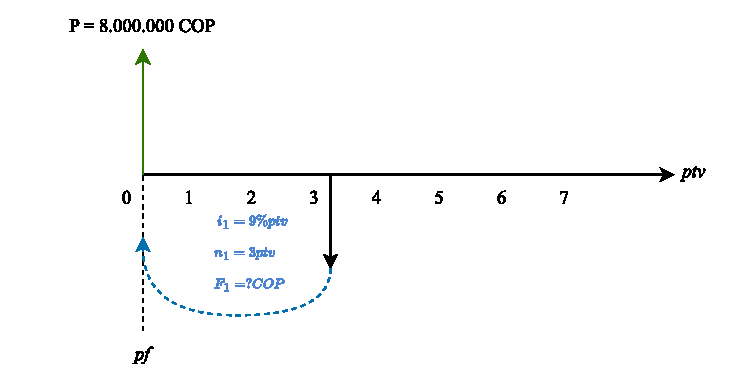
\includegraphics[trim=-5 -5 -5 -5 , max width=250px, max height=350px]{5_Capitulo/ejemplos/1/Capitulo5Ejemplo1-1.pdf}}\\
		\multicolumn{3}{|c|}{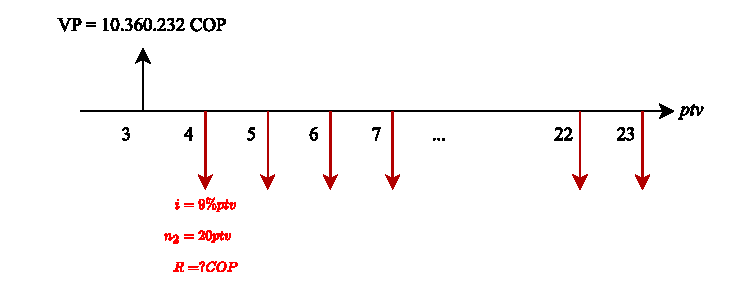
\includegraphics[trim=-5 -5 -5 -5 , max width=250px, max height=350px]{5_Capitulo/ejemplos/1/Capitulo5Ejemplo1-2.pdf}}\\ \hline
		%%%%%%%%%%%%% FIN INSERCIÓN DE IMAGEN<
		%%%%%FIN FLUJO DE CAJA
		
		
		
		%%%%% INICIO DECLARACIÓN FORMULAS
		%%%%%%%%%%% INICIO TITULO
		\rowcolor[HTML]{FFB183}
		\multicolumn{3}{|c|}{\cellcolor[HTML]{FFB183}\textbf{4. Declaración de fórmulas}}    \\ \hline
		%%%%%%%%%%% FIN TITULO
		%%%%%%%%%%% INICIO MATEMÁTICAS
		\multicolumn{3}{|c|}{$VP=R\cdot(\frac{1-(1+i)^{-n}}{i})\hspace{0.3 cm}\textit{Valor presente de una serie uniforme vencida}$} \\
		\multicolumn{3}{|c|}{$F=P(1+i)^{n}\hspace{0.3cm}\textit{Valor futuro}$}		
		\\ \hline
		%%%%%%%%%% FIN MATEMÁTICAS
		%%%%%% INICIO DESARROLLO MATEMÁTICO
		\rowcolor[HTML]{FFB183}
		%%%%%%%%%%INICIO TITULO
		\multicolumn{3}{|c|}{\cellcolor[HTML]{FFB183}\textbf{5. Desarrollo matemático}}       \\ \hline
		%%%%%%%%%% FIN TITULO
		%%%%%%%%%% INICIO MATEMÁTICAS
		\multicolumn{3}{|c|}{$F_{1}=8{.}000{.}000\,\,COP\cdot(1+0,09)^{-3}=10{.}360{.}232\,\,COP$} \\
		\multicolumn{3}{|c|}{$10{.}360{.}232\,\,COP=R\cdot(\frac{1-(1+0,09)^-{20}}{0.09})$} \\ \hline
		\multicolumn{3}{|c|}{$10{.}360{.}232\,\,COP=R\cdot(9,128545669)$} \\
		\multicolumn{3}{|c|}{$R=1{.}134{.}926,896\,\,COP$} \\
		\hline
		
		
		%%%%%%%%%% FIN MATEMÁTICAS
		%%%%%% FIN DESARROLLO MATEMÁTICO
		%%%%%% INICIO RESPUESTA
		\rowcolor[HTML]{FFB183}
		%%%%%%%%%%INICIO TITULO
		\multicolumn{3}{|c|}{\cellcolor[HTML]{FFB183}\textbf{6. Respuesta}}   \\ \hline
		%%%%%%%%%% FIN TITULO
		%%%%%%%%%% INICIO RESPUESTA MATEMÁTICA
		\multicolumn{3}{|p{\textwidth}|}{\centering{El valor de la cuota trimestral a cancelar es de $R=1{.}134{.}926,896\,\,COP$}}  \\ \hline
		%%%%%%%%%% FIN MATEMÁTICAS
		%%%%%% FIN RESPUESTA
	\end{longtable}
	%Se crean dos lineas en blanco para que no quede el siguiente texto tan pegado
	%\newline \newline %USARLO SI CREES QUE ES NECESARIO
\end{center}
%%%%%%%%%%%%%%%%%%%%%%%%%%FIN EJERCICIO 1 %%%%%%%%%%%%%%%%%%%%%%%%%%%
